% Chapter 5

\chapter{Component Selection \& Circuit Design} % Main chapter title
\label{Chapter5} % Change X to a consecutive number; for referencing this chapter elsewhere, use \ref{ChapterX}

\AddToShipoutPicture*{\CircuitDesign}

\begin{parcolumns}[colwidths={1=.6\textwidth},rulebetween=false]{2}
\colchunk{% left column

This chapter provides a detail description and insight into the derivation of the circuit design on the hardware requirements. 
This includes: (\ref{chap5sec1}) component selection, where for all the major components the method behind choosing the component is given; and (\ref{chap5sec2}) the circuit design, this section describes the method behind the circuit design for each of the various segments of the PCB. 

\section{Component Selection} 
\label{chap5sec1}
	
	This section describes the major components selected for the phone, note that most of the components were chosen based of previous student research \cite{Puranikthesis:report}.  
This process was completed before the circuit design was performed. 
This also includes other components which were compared and tested so that the optimal solution would be found. 

}
\colchunk{% right column
}
\end{parcolumns}
\newpage

%----------------------------------------------------------------------------------------
%	SECTION 1
%----------------------------------------------------------------------------------------

%----------------------------------------------------------------------------------------
%	SUBSECTION 1
%----------------------------------------------------------------------------------------

\subsection{Resistor and Capacitor Selection}

It was decided early on that (where possible) that all resistors and capacitors would be 0805 sized. 
This would maintain the aesthetic look of the PCB, as well as reduce hassle with the order and delivery of components. 
Most of the inductors on the board were also of 0805 size or of a similar size. 

%----------------------------------------------------------------------------------------
%	SUBSECTION 2
%----------------------------------------------------------------------------------------

\subsection{Power Supply Option}

	There were a number of different options that could have been chosen for the power supply. 
The proposed idea for the supply circuit was to have multiple power supplies for all the major components of the device. 
It was found through analysing the circuit after completing the main portion of the schematics that the current output would have to be at least 4A to account for the modems. 
However, in most circumstances the modems would probably still work fine with 2A. 
There were some issues trying to find a power supply option that both could output at least 2A of current and could be SMD soldered in a regular fashion. 

\subsubsection{TPS6302x High Efficiency Single Inductor Buck-Boost Converter}

It was proposed early on that multiple Texas Instruments TPS6302x High Efficiency Single Inductor Buck-Boost Converters with 4-A Switches would be used as the power supply. 
One was designed for both of the cellular radios, one to power WiFi and Bluetooth, one for the FPGA board, one connected to the battery source and two for the modems. 
This option was given priority over the other power supplies due to it having a 2A enable line, and after analysing the other power supply options was used as the power supply option. 


\subsubsection{CDMA Cellular/PCS System Power Supplies}

This power supply was considered however the power supplies are designed specifically for CDMA cellular/PCD handsets. For this reason, these power supplies were deemed to be not sufficient for the purposes of the phone. 

\subsubsection{TPS6128xA Low-, Wide- Voltage Battery Front-End DC/DC Converter Single-Cell Li-Ion, Ni-Rich, Si-Anode Applications}

The LP2951 voltage regulator was chosen as the regulator due to it having a low quiescent current and a low dropout voltage. The regulator also is ideally suited to work in battery-powered systems. 

\subsubsection{LP2951-N Adjustable Micropower Voltage Regulator}

The LP2951 voltage regulator was chosen initially as the regulator due to it having a low quiescent current and a low dropout voltage. 
It was also chosen as it was readily available and easy to obtain. 
The regulator also is ideally suited to work in battery-powered systems. 
Later on in the project it was found that the regulator didn't provide enough current to supply to the WiFi module and the modems, because of this an alternative was found which would supply the correct current.


\subsubsection{TPS63805 High Current, High Efficiency Single Inductor Buck-Boost Converter}

After discovering that the LP2951 voltage regulator wouldn't be sufficient for the project the TPS63805 was chosen instead as it would provide a high enough current to be able to work with both the two modems and the WiFi module. 
However, this module was in DSBGA form and was unsuitable for the device due to its soldering requirements. 


%----------------------------------------------------------------------------------------
%	SUBSECTION 3
%----------------------------------------------------------------------------------------

\subsection{4G Modem}
\subsubsection{ QUECTEL EC25-AU}

	This module was chosen based upon research completed by another student \cite{Puranikthesis:report}. 
This modem was also being used in the bench-top prototype, and already familiar with most of the software developed. 
%----------------------------------------------------------------------------------------
%	SUBSECTION 4
%----------------------------------------------------------------------------------------

\subsection{WiFi Module}
\subsubsection{Cypress BCM43362 WiFi + ST Micro STM32F405 MCU}
		This module was also chosen based upon research completed by another student \cite{Puranikthesis:report}.
Again, this module was already being used in the bench-top prototype and familiar with the software being developed for it. 

%	SUBSECTION 5
%----------------------------------------------------------------------------------------

\subsection{Bluetooth Module}
\subsubsection{RN52 Module}
	This module was chosen based of its use for simple, mobile devices and its cost. 
There weren't many other alternatives that provided the same features. 
This module's schematic was rather simple to implement with the datasheet providing a layout for the footprint for the component.

%----------------------------------------------------------------------------------------
%	SUBSECTION 6
%----------------------------------------------------------------------------------------

\subsection{LoRa Module}
\subsubsection{RN2483 LoRa Module}
	This module was also chosen based upon research completed by another student \cite{Puranikthesis:report}. 

%----------------------------------------------------------------------------------------
%	SUBSECTION 7
%----------------------------------------------------------------------------------------

\subsection{Battery Charger}
\label{chap:charger}
\subsubsection{BQ25071}
	This module was chosen based upon previous research \cite{Puranikthesis:report} and was found to work well with the MicroUSB connection to be used on the phone. 
		
%----------------------------------------------------------------------------------------
%	SECTION 2
%----------------------------------------------------------------------------------------

\section{Designing the Schematics}
\label{chap5sec2}

	All of the following schematics that will be mentioned in this section were designed using Altium Designer 18. 
The use of component data sheets and online tutorials aided in the design as well as input from the Academic Supervisor. 
Most of the schematic and PCB models were either downloaded from the manufacturer's website or from SnapEDA. 
The following paragraphs will give an overview of the various schematics and why they were designed and for what purpose they have with the MEGA65 phone.

\subsection{FPGA Pins}
\label{chap:FPGA}
	The FPGA pins were designed to be connected to the Nexys FPGA board and are the sole CPU of the device. 
This part of the device will have the Nexys FPGA board plugged into the top of it.\\
Being the overall connection sheet for the phone, the FPGA pin sheet was labelled as the top sheet. 
The FPGA would be the main CPU of the board with most components on the phone needing a connection to an FPGA pin. 
Two 50-Pin headers were placed on the schematic which mimicked the pin connection on the FPGA board. 
Some of the connections to other components included the I2C connections (data and clock lines), PCM connections, UART connections and the red, green and blue connections for both the VGA connection and LCD screen.\\
The schematic of the component was designed for the project while the footprint was found pre-made.\\
Figure \ref{fig:header} displays one of the 50-pin headers which connect to the FPGA.

\begin{figure}
	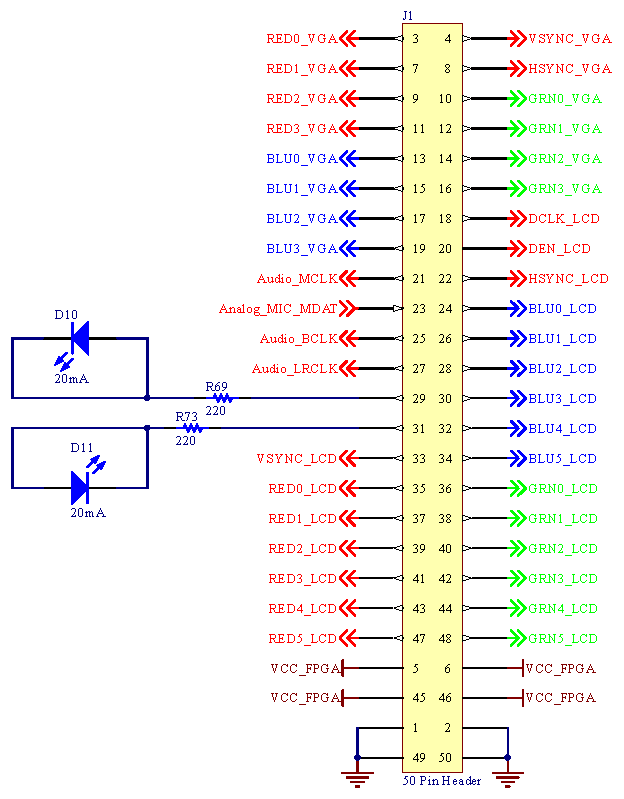
\includegraphics[width=0.5\linewidth]{Figures/50_pin_header.pdf}\centering
	\caption{Schematic of 50-pin Header}
	\label{fig:header}
\end{figure}

\subsection{Power Control Circuitry}
\label{chap:batt}
	The Power Control circuitry was designed to ensure that certain devices could be switched off if required, and also to ensure that adequate power was being supplied to all necessary components on the device. 
To begin a number of voltage regulators were added to the schematic as well as a flip-flop to be used for the main FPGA power. 
A I2C I/O Expander was also used in the schematic so that all the voltage regulators could be connected to it.\\

	The circuitry was connected up by first connecting a slide switch between the shutdown and power lines of the voltage regulator. 
An LED was then connected to the output line to ensure that if the regulator was powered an LED would illuminate, with the output line producing the required power rail needed. 
This was repeated six times to create the multiple power rails required for all the different components.\\

	There were a few changes made to the power control circuitry after going through and analysing all the schematics. 
It was found that the voltage regulator would only give out 0.1A of current whereas the modems would need at least 2A of current, 4A at best. 
The circuitry was updated to include the new part found so that the output current would be adequate for the modems. \\

\subsection{Charging Circuitry}

	The charging circuit was designed using a Bq25071 chip connected to a MicroUSB connector. 
The charging circuit chip was set to be powered by the battery voltage line. The circuitry was designed following the datasheet of the IC.
Figure \ref{fig:charger} displays the charging circuit with the MicroUSB connection to the left. 

\begin{figure}
	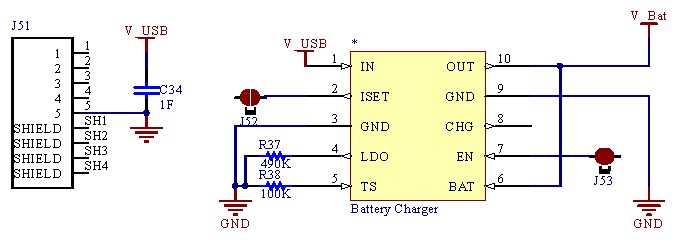
\includegraphics[width=0.5\linewidth]{Figures/battery_charger.pdf}\centering
	\caption{Schematic of Charging Circuit with MicroUSB connection}
	\label{fig:charger}
\end{figure}

\subsection{Voltage Step-Up \& Step-Down}

	The Voltage Step-up was required as a few of the components require 5V. 
This was completed by using an NCP1402 and connecting VCC MIC to the input voltage line. 
The rest of the circuitry was completed by following the recommended layout in the data sheet. 
The use of the NCP1402 was based on a recommendation written in a past student's thesis, with the component being verified for its usability in the phone. 
An LP5951 was used to step the voltage down from 3.3V to 1.3V for the required components which needed this voltage. 
Figures \ref{fig:stepup} and \ref{fig:stepdown} display the schematics for both the voltage step-up and step-down circuits.

\begin{figure}
	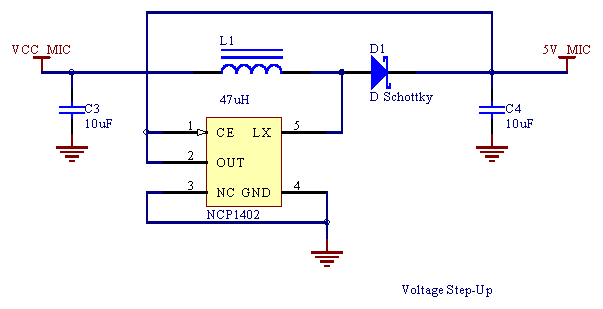
\includegraphics[width=0.5\linewidth]{Figures/voltage_stepup.pdf}\centering
	\caption{Schematic of Voltage Step-Up}
	\label{fig:stepup}
\end{figure}

\begin{figure}
	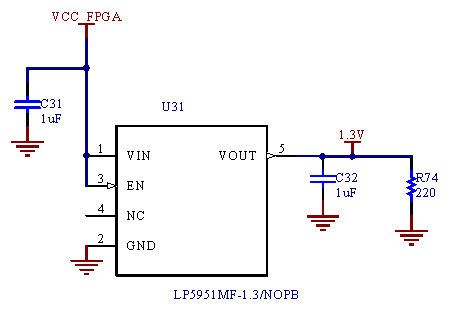
\includegraphics[width=0.5\linewidth]{Figures/voltage_stepdown.pdf}\centering
	\caption{Schematic of Voltage Step-Down}
	\label{fig:stepdown}
\end{figure}

\subsection{Signal Connections}

	The Signal Connections schematic was designed to contain all the off-sheet connectors from the various components which operated through I2C and Interrupt lines. 
The separate signals were connected together with resistor pull-ups added to the two I2C lines. 
The output of these signals were all sent directly to FPGA pins. 
Figure \ref{fig:SCL} displays the schematic for the SCL connections. 

\begin{figure}
	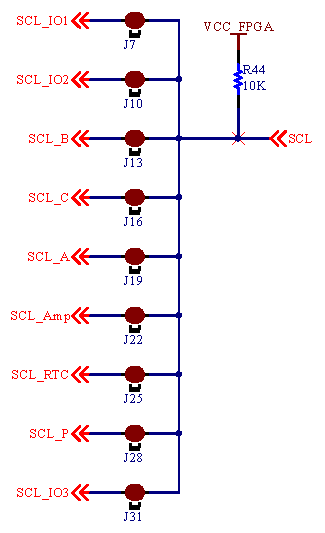
\includegraphics[width=0.5\linewidth]{Figures/SCL_lines.pdf}\centering
	\caption{Schematic of SCL connections}
	\label{fig:SCL}
\end{figure}


\subsection{I2C I/O Expanders}

	There were a number of I/O Expanders which were added to the device. These were added to add in a number of peripherals which didn't necessarily need to be connected to FPGA pins. There were a number of expanders due to all the pins on a particular expander needing to have the same inout/output source. 
The I/O Expanders were added into the schematics to allow the device to have more connections. The DPAD and buttons were connected to an I/O Expander with the use of resistor pull-ups. A number of other signals which were required to be active while the FPGA was active, were added to another I/O Expander.
Figure \ref{fig:I2C} displays the schematic for one of the I2C Expanders. 

\begin{figure}
	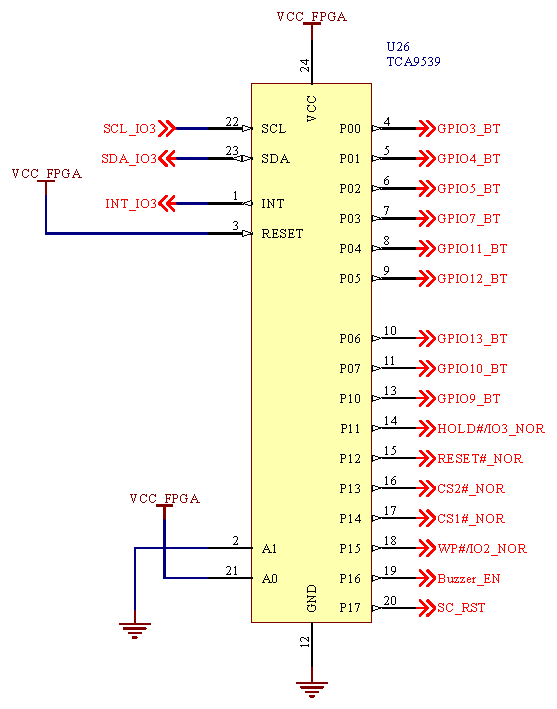
\includegraphics[width=0.5\linewidth]{Figures/I2C_Expander.pdf}\centering
	\caption{Schematic of I2C Expander}
	\label{fig:I2C}
\end{figure}

\subsection{VGA Connection}
\label{chap:VGA}

	The VGA was connected using a 15-Pin DSUB connector. 
A resistor ladder was used for the colour connections with the signals going straight out to the FPGA board.
Resistor values of 4k, 2k and 510 Ohms were used for the ladder with two 0 Ohm resistors used for the HSYNC and VSYNC lines. 
The data sheet for the VGA connection was used as a basis for the signal connections. 
Figure \ref{fig:VGA} displays the VGA connection. 

\begin{figure}
	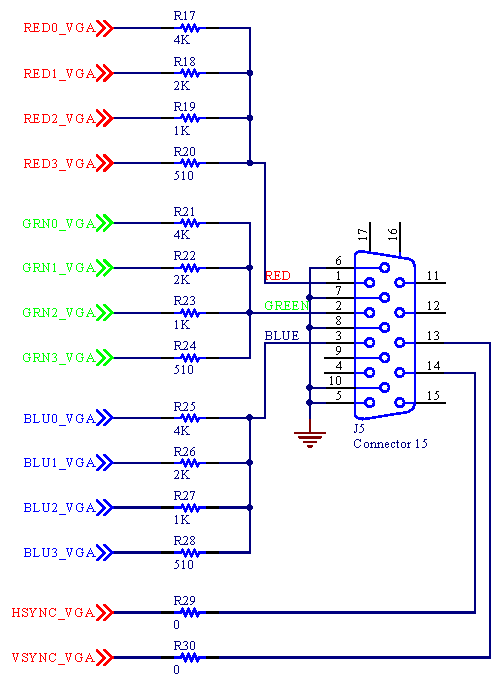
\includegraphics[width=0.5\linewidth]{Figures/VGA.pdf}\centering
	\caption{Schematic of VGA Connection}
	\label{fig:VGA}
\end{figure}

\subsection{LCD Display}
\label{chap:LCD}

	The LCD Display schematic was connected in a similar way as the VGA connection with resistor pull-ups used for all three colour connections. 
The purpose of the schematic would be to provide the LCD display for the phone.
Figure \ref{fig:LCD} displays the LCD connection.

\begin{figure}
	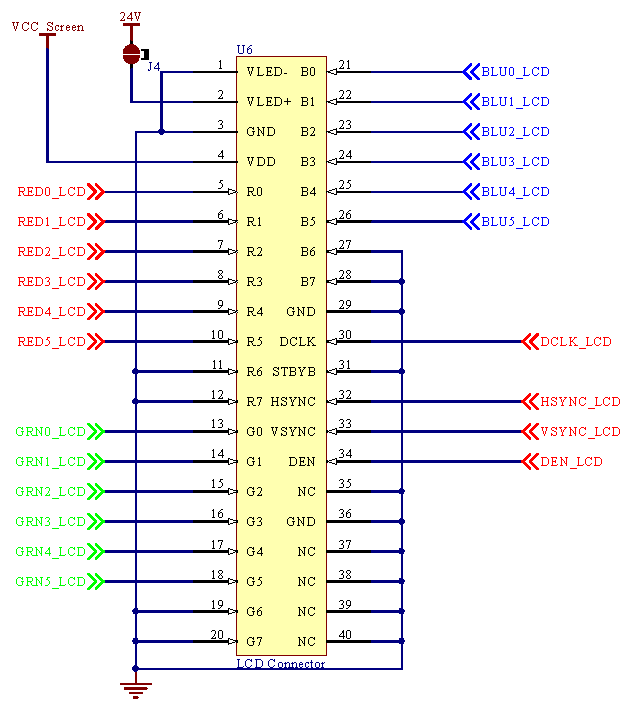
\includegraphics[width=0.5\linewidth]{Figures/LCD.pdf}\centering
	\caption{Schematic of LCD Screen Connection}
	\label{fig:LCD}
\end{figure}

\subsection{Touch Screen}
\label{chap:touch}

	The Touch Screen was added to the schematic to give the ability to the user to use their fingers for functionality, as well as the thumb-pad and buttons. 
The Touch Screen connection was completed by powering it with VCC Screen and adding in I2C signals and an Interrupt line, going to the Signal Connections sheet.

\subsection{LED Backlight Display}

	The LED Backlight Display was designed using a simplified design already created by another producer. This circuit was designed to provide a back lit display when the phone is on and to dim the screen when the phone is in a call or facing down.
Figure \ref{fig:backlight} displays the LED Backlight connection. 

\begin{figure}
	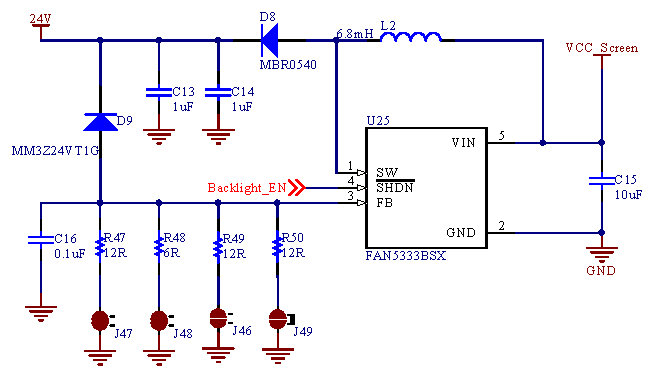
\includegraphics[width=0.5\linewidth]{Figures/LED_backlight.pdf}\centering
	\caption{Schematic of the LED Backlight Connection}
	\label{fig:backlight}
\end{figure}

\subsection{Accelerometer}
\label{chap:a}

	The accelerometer was designed mainly through reading the recommended application layout in the data sheet of the component. Off-sheet connectors were used for the I2C signals and the Interrupt lines, as well as the three ADC lines which were used for the volume thumb wheel. The power for the component was connected to the VCC MIC power rail.
Figure \ref{fig:a} displays the accelerometer connection. 

\begin{figure}
	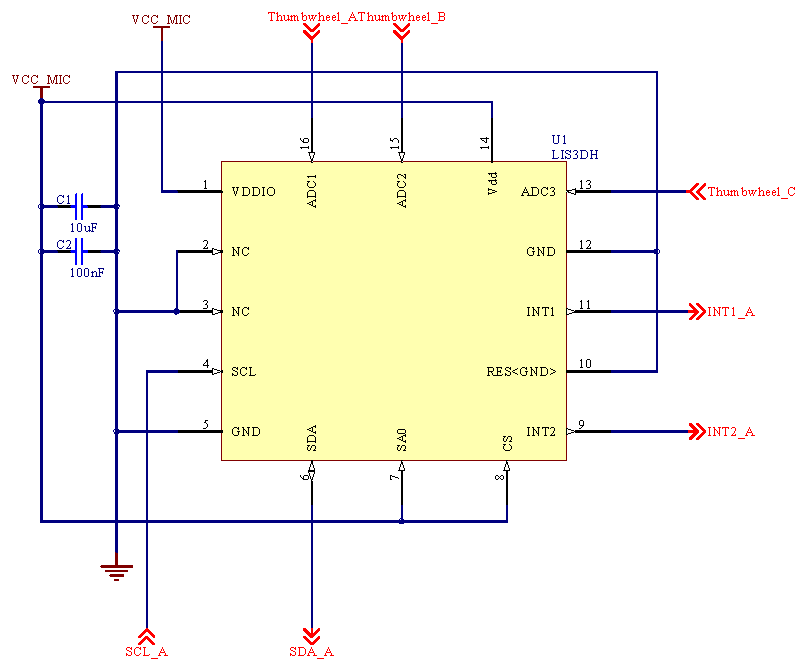
\includegraphics[width=0.5\linewidth]{Figures/accelerometer.pdf}\centering
	\caption{Schematic of the Accelerometer Connection}
	\label{fig:a}
\end{figure}

\subsection{Real-Time Clock}
\label{chap:RTC}

	The schematic connections for the RTC were made by following the typical application layout given in the manufacturer's data sheet.
Figure \ref{fig:RTC} displays the real-time clock connection. 

\begin{figure}
	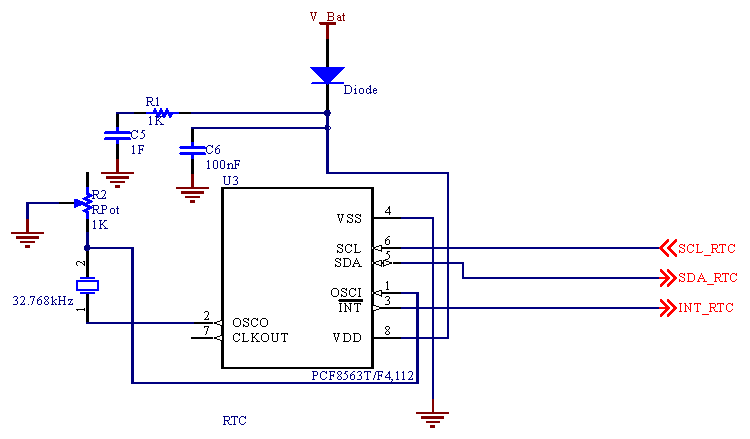
\includegraphics[width=0.5\linewidth]{Figures/RTC.pdf}\centering
	\caption{Schematic of the Real-Time Clock Connection}
	\label{fig:RTC}
\end{figure}

\subsection{Proximity Sensor}
\label{chap:prox}
	The schematic and PCB models for the Proximity Sensor were accessed from the internet with all the connections followed from the manufacturer's data sheet. 
Figure \ref{fig:prox} displays the proximity sensor connection. 

\begin{figure}
	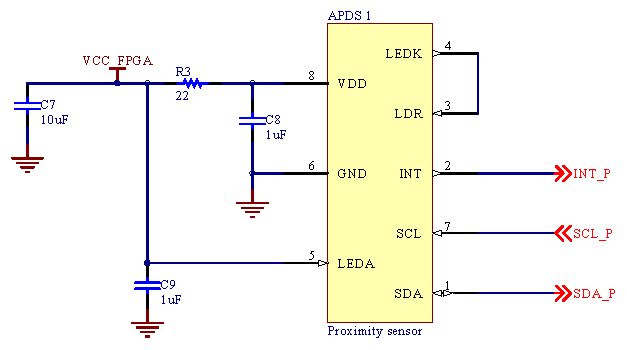
\includegraphics[width=0.5\linewidth]{Figures/prox_sensor.pdf}\centering
	\caption{Schematic of the Proximity Sensor Connection}
	\label{fig:prox}
\end{figure}

\subsection{4G Modems}
\label{chap:modem}

	4G modems were added to the device to enable 4G internet connection. 
Two 4G modems were added to the schematics so that the user would have the ability to be connected to two different networks at once.
The schematic for the 4G modem was downloaded off the internet with many of the connections also being read off the manufacturer's data sheet. 
Figure \ref{fig:modem} displays the 4G modem connection. 

\begin{figure}
	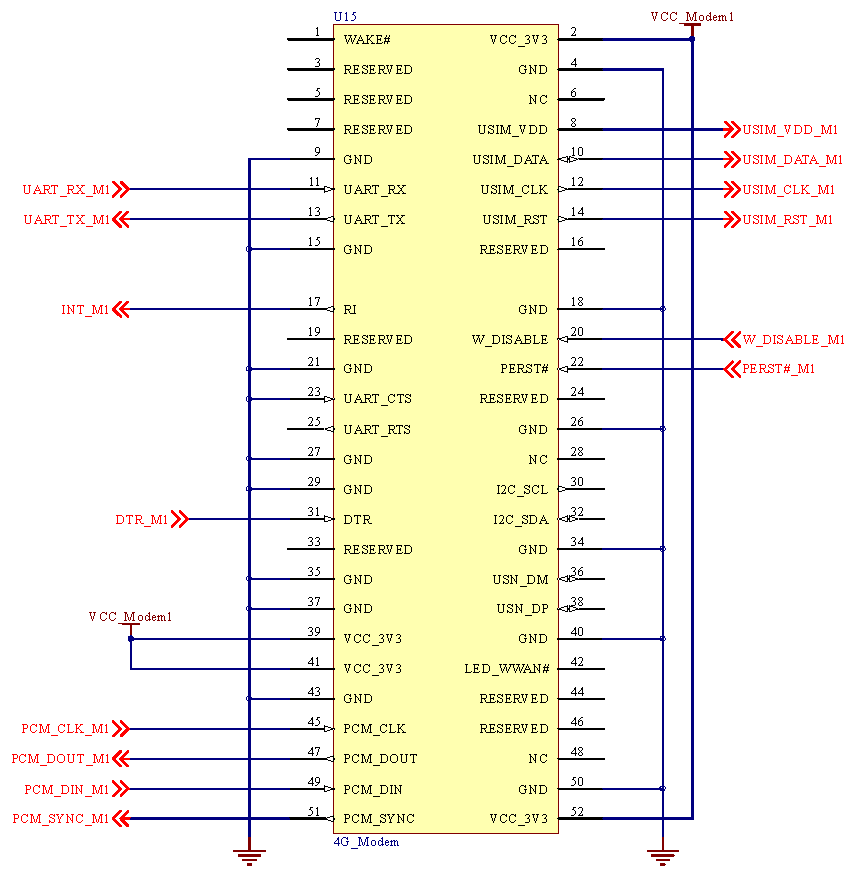
\includegraphics[width=0.5\linewidth]{Figures/modem.pdf}\centering
	\caption{Schematic of the 4G Modem Connection}
	\label{fig:modem}
\end{figure}

\subsection{WiFi Module}

	The WiFi module was added into the schematics to enable the phone to have WiFi capability. This module was connected through the GPIO bits and an I2C connection.

\subsection{NOR Flash}

	The NOR Flash schematic was designed to have primary use within the One-Time Pad encryption. The component would have no other function on the phone. 

\subsection{Barometer}

	The schematic connections for the Barometer were completed by following the recommended layout given on the manufacturer's data sheet. 
Figure \ref{fig:barometer} displays the schematic for the barometer. 

\begin{figure}
	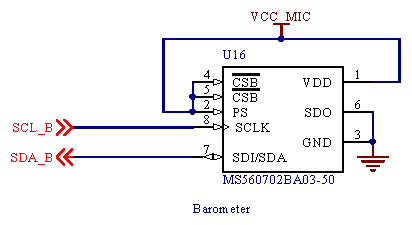
\includegraphics[width=0.5\linewidth]{Figures/barometer.pdf}\centering
	\caption{Schematic of the Barometer}
	\label{fig:barometer}
\end{figure}

\subsection{LoRa Radio}

	The two LoRa Radios were connected up using the recommended application layout given by the manufacturer's data sheet. 
The UART connections were made directly to the FPGA pins. 

\subsection{MEMs Microphones}
\label{chap:mics}

	The two MEMs Microphones were connected by following the data sheet's guidelines. The individual data lines were sent straight to the FPGA, while the two clock lines were tied together and sent to the FPGA board. 

\subsection{Headphone Audio Filter} 
\label{chap:audio2}

	The Headphone Audio Filter was created by following the design of a Sallen-Key Lowpass Filter, with two being designed. A chip containing two amplifiers was used for the design with the output of both chips being the left and right headphone audio respectively. 

\subsection{Audio Power Amplifier}
\label{chap:audio}

	The schematic for the Audio Power Amplifier was completed using a number of recommended layouts found in the component's recommend layout and recommended schematics found across the internet. This schematic was designed to produce the audio for the phone. 
Figure \ref{fig:audio} displays part of the audio circuitry. 

\begin{figure}
	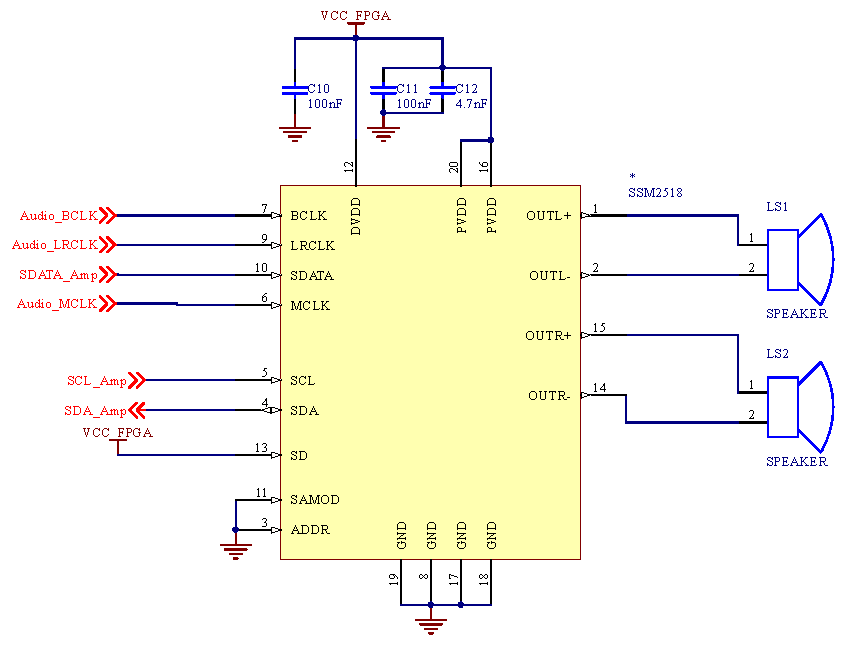
\includegraphics[width=0.5\linewidth]{Figures/audio_circuitry.pdf}\centering
	\caption{Schematic of part of the Audio Circuitry}
	\label{fig:audio}
\end{figure}

\subsection{Digital Compass}

	The Digital Compass was added to give the device the use of a compass which would be used for both gyroscopic effect and the location of the device.
Like many of the other components the signal connections on the schematic were wired using the recommended application layout. 
Figure \ref{fig:compass} displays the schematic of the digital compass. 

\begin{figure}
	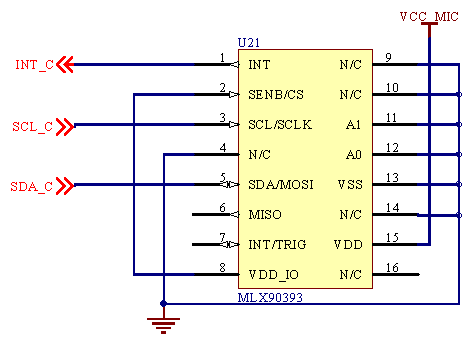
\includegraphics[width=0.5\linewidth]{Figures/compass.pdf}\centering
	\caption{Schematic of the Digital Compass}
	\label{fig:compass}
\end{figure}

\subsection{Bluetooth Module}

	The Bluetooth module was added into the schematic to ensure that the device would be compatible with Bluetooth. This would allow the user to connect to a third-party peripheral device.
The circuitry for the Bluetooth module was created by following the recommend layout on the component's data sheet. The UART and PCM connections were made directly to FPGA pins. 

\subsection{SIM Card Connection}
\label{chap:SIM}

\subsection{MicroSD Card Slot}
\label{chap:SD}

	The MicroSD connection was created by downloading a MOLEX schematic and footprint from SnapEDA. The data, clock and chip select lines were connected to the FPGA directly with a 100k$\Omega$ pull-up resistor for every signal. The structure for the pull-up resistors was followed from a Nexys 4 DDR schematic sheet created by Digilent. 

\subsection{Smart Card Connection}
\label{chap:SC}

	The Smart Card Connection was created by designing a custom footprint and schematic. 
The footprint was drawn based off the Smart Card Slot datasheet, with the schematic being a basic header block with ten connections.\\
The Smart Card was implemented to allow the user to make payments with their phone, without having to pull out their credit/debit card.
Figure \ref{fig:SC} displays the schematic for the Smart Card Connection. 

\begin{figure}
	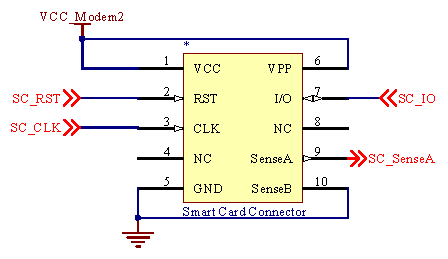
\includegraphics[width=0.5\linewidth]{Figures/SC.pdf}\centering
	\caption{Schematic of the Smart Card Connection}
	\label{fig:SC}
\end{figure}

\subsection{Buzzer}
\label{chap:buzzer}

	The buzzer was added to allow notifications whenever a text or missed call was recieved.
Figure \ref{fig:buzzer} displays the schematic for the buzzer. 

\begin{figure}
	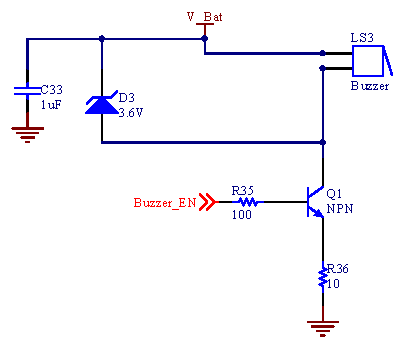
\includegraphics[width=0.5\linewidth]{Figures/buzzer.pdf}\centering
	\caption{Schematic of the Buzzer Connection}
	\label{fig:buzzer}
\end{figure}

%----------------------------------------------------------------------------------------


